%\documentclass{article}
\documentclass[a4paper,11pt]{article}
\usepackage[utf8]{inputenc}
\usepackage{graphicx}
\usepackage{url}
\usepackage{float}
\usepackage{times}
\usepackage{multirow}
\usepackage{listings}
\usepackage{times}
\usepackage{paralist}
\usepackage{epsfig}
\usepackage{subfigure}
\usepackage[hypertex]{hyperref}
\usepackage{subfigure}
\usepackage{color}

%\documentclass{rspublic}

\usepackage{ifpdf}

\newcommand{\I}[1]{\textit{#1}}
\newcommand{\B}[1]{\textbf{#1}}
\newcommand{\BI}[1]{\textbf{\textit{#1}}}
\newcommand{\T}[1]{\texttt{#1}}

\pdfpagewidth 8.5in
\pdfpageheight 11in 

\setlength\topmargin{0in}
\setlength\headheight{0in}
\setlength\headsep{0in}
\setlength\textheight{9in}
\setlength\textwidth{6.5in}
\setlength\oddsidemargin{0in}
\setlength\evensidemargin{0in}
\setlength\parindent{0.1in}
\setlength\parskip{0.25em}

\ifpdf
 \DeclareGraphicsExtensions{.pdf, .jpg}
\else
 \DeclareGraphicsExtensions{.eps, .ps}
\fi

\newif\ifdraft
\drafttrue

\ifdraft
\newcommand{\fixme}[1]{ { \bf{ ***FIXME: #1 }} }
\newcommand{\jhanote}[1]{ {\textcolor{red} { ***Jha: #1 }}}
\newcommand{\yyenote}[1]{ {\textcolor{blue} { ***yye00: #1 }}}
\else
\newcommand{\jhanote}[1]{}
\newcommand{\yyenote}[1]{}
\newcommand{\fixme}[1]{}
\fi

\begin{document}

\title{\large Implementing Abstractions for Data Intensive Applications using SAGA}

\author{Christopher Miceli$^{1}$, Michael Miceli$^{1}$, Bety Rodriguez-Milla$^{1}$, Shantenu Jha$^{1,2}$\\
  \small{\emph{$^{1}$Center for Computation \& Technology, Louisiana State University, USA}}\\
  \small{\emph{$^{2}$Department of Computer Science, Louisiana State
      University, USA}}}

\maketitle

\section{New Abstract}

There is a need for abstractions to support data-intensive computing, and these abstractions are required at several levels -- programmatic, system and data-access patterns.  As data volumes increase, it is often impossible to store data ``locally''. In addition to just storage, often the data consumed by a single application is produced at multiple distributed sites (think sensors).

There are at least two types of data-intensive applications: the first where the actual data generated is large; the second type is where the data generated is small, but the volume of data on which computation occurs is very large. \jhanote{Can you elaborate on different types of data-intensive applications? What kind is
an ImageMagic based application?}

\jhanote{The assumption in the next sentence is that all Data Intensive applications are distributed, thus add the word, ``Distributed''.} Data intensive grid applications need to be very mindful of the location of the data being operated on.  In some cases, moving data to a distributed source of computation may be advantageous, compared to utilizing the computation resource co-located with the data (volume of data might be very large thus multiple threads of compute, or I/O requirements might be very large, thus saturating I/O channels). In general, the traditional (simple) assumptions of data being shipped to whereever the computation was to occur are no longer valid. What are the factors that determine the movement of data, computation or both?
\jhanote{Address this question. (i) application type, (ii) infrastructure used, (iii) degree of distribution .. }

To understand the landscape of the challenges associated with developing and deploying Data-Intensive Applications, we have developed a framework that implements the well known All-Pairs Patterns, and we utilize this framework to perform Image Matching, where individual elements can be placed over different 
distributed resources.

Distributed filesystems % are a tool for grid developers that
simplying data-management problems such as replication and fault tolerance, allowing the application to focus on the problem it aims to handle. Certain problems, though, have certain specific properties that may be better handled if the application focused on data management.  Amongst other things, in this paper, we will analyze the performance trade-offs when using distributed filesystems for grid applications, compared to manual data placement and handling.

In this paper we use an grid-enabled all-pair algorithm application.  This application applies an operation on the input data set such that every pair in the set will be input to the operation.  The result of this application is stored in a matrix.  This application spawns jobs on the grid to run sets of these pairs.  The problem becomes determining which pairs to put into a set, and which distributed resource to run that set.  If transferring data to the grid job takes too long, we will spend more time on data management than computation.  There may be an entity in the grid capable of the work that may be slower than others, but close enough to the data to make up for its lack of computational ability.

Distributed filesystems replicate files across data stores to provide fault-tolerance and improve performance by dishing data out from the closes source.  In our experiments, we used CloudStore, an open-source high performance distributed filesystem that builds upon ideas from Google's distributed filesystem GFS.  CloudStore was chosen for its high performance focus, C++ implementation, and its source code availability.

\jhanote{references needed. for example, CloudStore, All-Pairs, KFS.. }

We use the results of three different experiments when determine the utility of distributed filesystems.  In the first experiment, we run our all-pairs application on a grid without regard to data placement.  This means that the application will naïvely assign a job to perform operations on data without regard to where the data being operated on is located in the grid.
The second experiment will be similar to the first, except the all-pairs application will take the data's location into consideration when determining whether or not to assign a certain data set to a job. This version of the application performs an extra step that determines the performance of the grid by pinging hosts that may be involved, and utilizes this information when deciding which data set to assign to a job requesting work.  \jhanote{OK to start off with ping, but something more sophisticated than ping will be required. Use iperf? or other similar tools (netperf?)}  If there is an unprocessed data set collocated or network-close with the job, then the assignment of that worker to that data set would have benefits.  If there is no unprocessed data set network-close to the job, still assign data that may be network-far, in case the network-close job failed or there is no available jobs network-close to the data set.

The third experiment will provide information into distributed filesystem's performance in handling data locality issues.  \jhanote{What about replication factor as a variable of the experiment?}  The all-pairs application will be the same as the first, except all data will be stored in the distributed filesystem CloudStore.  All read and writes will also utilize the distributed filesystem.  The performance of this test will be dependent on where the distributed filesystem is in relation to the jobs that will perform the work.  Our setup involved making block-servers on every machine that may be capable of performing work.  This will put all responsibility on the DFS in determining where to place data.
Notably, the second experiment is also naïve in the way that it attempts to optimize data and work assignments.  Recent work has shown that data in large scale grid applications tends to be accessed together, despite being seemingly unrelated in the data set.  The data accessed frequently together being called a filecule \jhanote{reference!}.  Attempting to determine these filecules in the all-pair application would be very difficult \jhanote{filecules -- or the lack thereof, are application specific, and possible compute-function dependent}. The distributed filesystem, while not being written for this purpose, will replicate files to chunkservers requesting that data frequently.  If the chunkserver is also capable of data processing, then the dfs will be placing filecules together, and on machines needing them for work.  The fault tolerance that distributed filesystems are already well renowned for also have added benefits to grid application developers.  The grid application does not have to be aware of where data has been copied to previously when assigning work.  The distributed filesystem will use the best data replica when data is being accessed.

The tests we run to determine the affect of distributed filesystems was to run tests using a version of the all-pairs application that attempts no data management optimizations, a second version that attempts many data management optimizations, and a third version third version that utilizes a distributed filesystem.  The first test will be a baseline to determine how a naïve approach would perform, even if this results in lengthy data transfer times throughout the grid.  The second test will demonstrate how well an application can perform when tailored to the specific problem at hand.  The third tests is to see if a distributed filesystem is able to perform on par with a highly tailored application.  If the distributed filesystem performs well, then a grid application developer will be able to spend less time 

\jhanote{Ok, so what? Need a few sentences, outlining the importance of this work and where
things stand and/or where things will go?}

\section{Old Abstract}

% For example, the power of Google is based upon a simple programming
% abstraction -- MapReduce~\cite{mapreduce}.  MapReduce is a framework
% for splitting up large data and keeping track of which machine the
% data is on. The purpose is to automatically parallelize and execute on
% large clusters.  The application itself has to provide only the
% specific map and reduce steps, reusing the bulk of the functionality
% from the provided generic implementation.  By relieving the
% end-developer from having to control explicitly data placement, job
% distribution, load balancing, etc., MapReduce provides a level of
% abstraction that simplifies the task of an application programmer.

\jhanote{Unclear if next 3 paragraphs should go?}

There exist additional powerful abstractions, such as AllPairs~\cite{allpairs}, which is both a programming abstractions and a system-level abstraction.  Allpairs is a framework for when every element of some data needs every other element of another set of data.  When implemented on distributed infrastructure, AllPairs, like MapReduce, essentially decouples the client's code from grid specific information.  Again, all the application has to provide is the ordering criteria of the data to work on, resuing the programming abstractions as implemented by the based framework.

SAGA~\cite{saga_gfd90} is a high level API that provides a simple,
standard and uniform interface to the most commonly required
distributed functionality.  SAGA can be used to encode grid
applications~\cite{saga_escience07, saga_tg08}, tool-kits to manage
distributed applications as well as implement abstractions that
support commonly occurring programming, access and usage patterns.
The focus of this paper is on the latter set, i.e.  the use of SAGA in
implementing well known abstractions for data intensive computing.

In this paper, we will implement MapReduce and All-Pairs abstractions
using SAGA and use them to solve commonly encountered genomic tasks.
We will show how multiple sequence alignment can be orchestrated using
the SAGA-Allpair implementation, and genome searching can be
implemented using Map-reduce.  In addition, the aim of this paper is
to show (validate) that SAGA is a sufficiently complete and high-level
interface so as to support these programming abstractions.

Figure~\ref{fig:data_intensive_app_saga} illustrates the software
architecture of the implementation, highlighting the different
abstraction levels that allow the reuse of most of the system for both
algorithms and for different genomic applications.  We will highlight
the sailent points of our implementations, and how we handle common
considerations such as when to move the data to the machine or when to
process it locally.  The implemention of these abstractions
encapsulates details such as latency hiding, performance and other
variables (such as cluster sizes, and queue sizes).  The user should
be able to easily add a few function calls without worrying about many
considerations required by most grid computing applications.

We will discuss other performance issues that arise when implementing
abstractions specific for data-intensive computing.  A grid
application's design should not focus on the bandwidth of the network,
the dispatch latency, the number of machines available, and data
reliability.  Even something as simple as process size can be a tough
challenge to optimize.  If a job is too small, then network traffic
becomes a bottleneck and the design is inefficient.  If a job is too
large, it is difficult to tell when it is hanging or still computing.
Also, if another job with a higher priority takes a machine over, the
application will be waiting on jobs longer.  The main point of this
paper is to show how a flexible, extensible implementation of
programming data-intensive abstractions using SAGA can shield the
application developer many of these considerations.

%these that can serve as a basis for data intensive applications.

% the mapreduce framework as well as a good guide for parallel
% programming.

% \begin{figure}
% \begin{center}
% 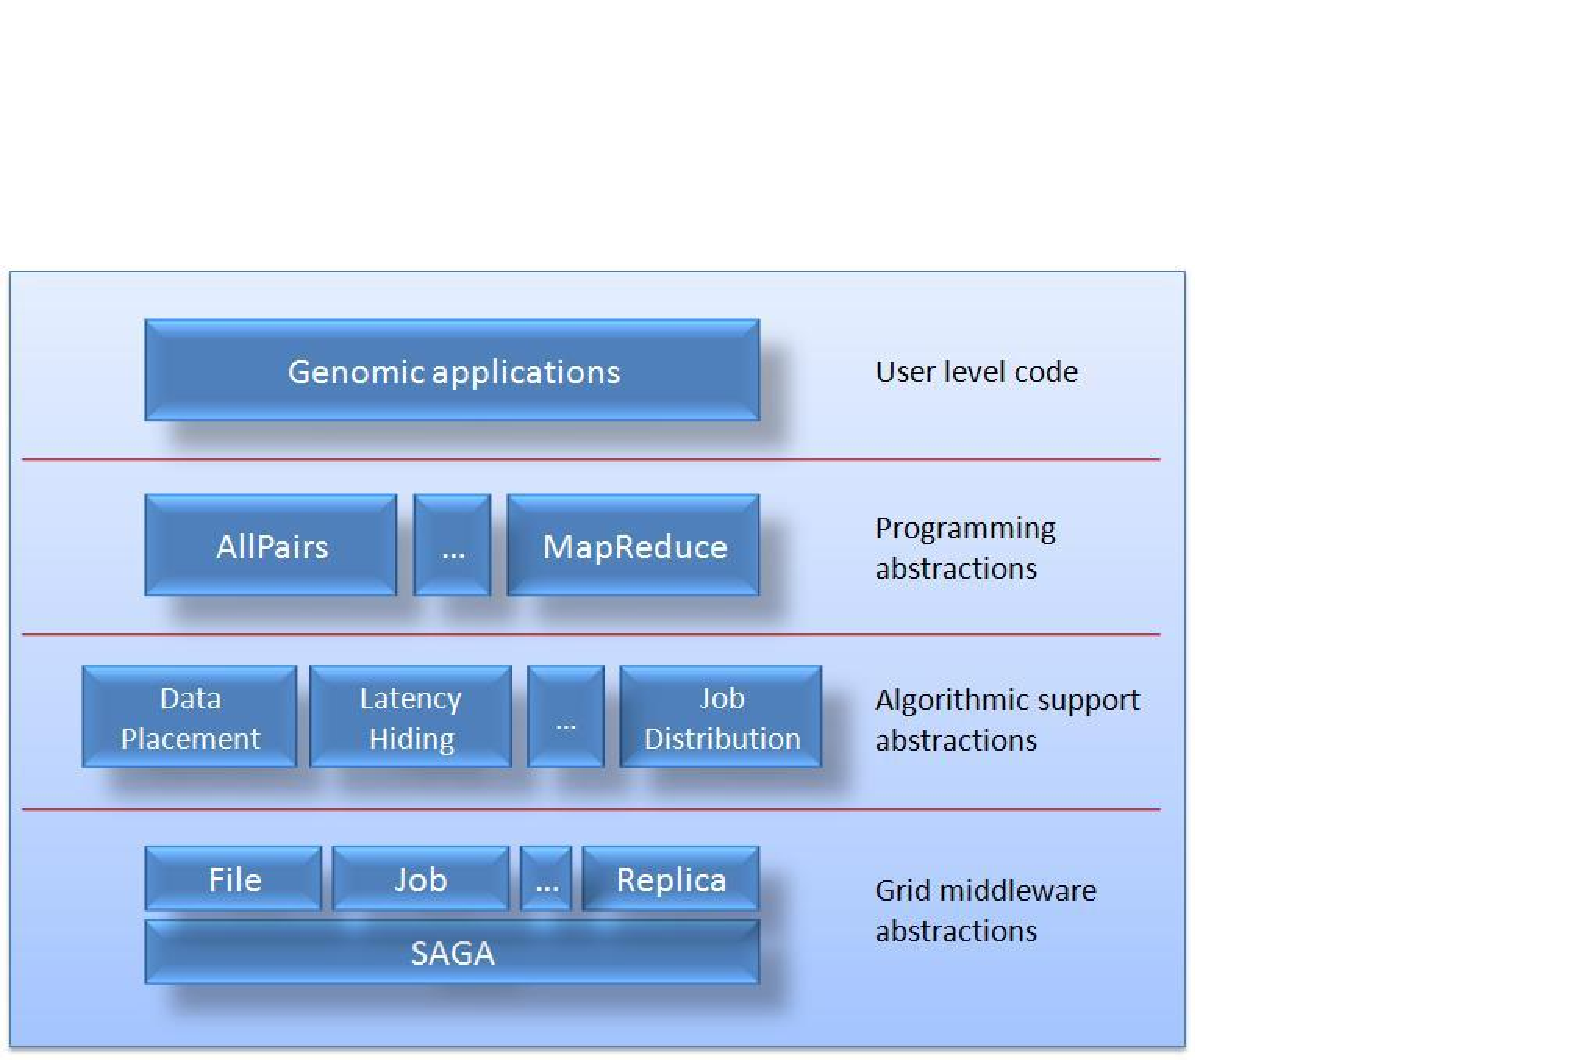
\includegraphics[scale=0.60]{data_intensive_app_saga}
% \end{center}
% \caption{The programming abstractions provided by the AllPairs and
%   MapReduce algorithm implementations are sufficient to enable a wide
%   range of genomic aplications (sequence alignment, searching, etc.)
%   to be distributed over grids. The required underlying functionality
%   is provided by higher level algorithmic support abstractions, such
%   as tools for data placement, latency hiding, and job distribution,
%   which ar ebeing built on top of grid middleware abstractions
%   provided by SAGA (such as file transfer, job launching, information
%   services and replica management.}
% \label{fig:data_intensive_app_saga}
% \end{figure}

\bibliographystyle{IEEEtran} 
\bibliography{saga}
\end{document}



% Distributed mergesort is an important example that can be used in many
% distributed applications. \ It encompasses all 4 phases of designing a
% successful parallel algorithm: \ partitioning, communication,
% agglomeration, and mapping. \ By designing and implementing a flexible
% implementation of distributed mergesort, different design and
% performance issues can be understood. \ Also, mergesort is a building
% block for mapreduce, a software framework for parallel computations on
% large data sets.


% Explore different implementations and the costs/benefits of each. \
% The broadest of implementation considerations is to use either a
% simple distributed mergesort or parallel mergesort. \ A simple
% distributed mergesort would have one central machine that receive data
% from many machines and merges all of the sorted pieces. \ Another
% implementation would be parallel mergesort. \ This involves sending
% pieces to many machines and have them communicate with its neighbors
% until all have of the machines have an equal sorted and merged
% sequence.
% There are many different ways to implement map reduce and each way has
% special considerations.  

%Map Reduce~\cite{mapreduce} and All-Pairs~\cite{allpairs}.
